\chapter{Introduction}
\label{ch:introduction}

\dictum[Albert Einstein]{%
   If you can’t explain it simply, you don’t understand it well enough.}
\vskip 1em

% \begin{otherlanguage}{ngerman}
% Die ältesten Bestimmungen der wahren Grösse der Moleküle hat die kinetische
% Theorie der Gase ermöglicht, während die an Flüssigkeiten beobachteten
% physikalischen Phänomene bis jetzt zur Bestimmung der Molekülgrössen nicht
% gedient haben. \dots
% \end{otherlanguage}


\section{Geothermal fields}
The Earth's interior contains vast amounts of thermal energy, primarily originating residual heat from planetary formation, magmatic activity, and other physical reactions \citep{leyton2017earth, lay2008heat}.
While the heat slowly dissipates towards the surface (gradient $\sim$\SI{25}{\celsius\per\kilo\metre}; \cite{dipietro2013gradient}), magmatic intrusions in the crust locally disrupt this gradient, creating temperature anomalies.
These intrusions are particularly common at plate boundaries, where subduction, rifting, and faulting facilitate magma ascent \citep{elders2025geothermal, hochstein1998plates}.
Additionally, radiogenic decay of U, Th, and K in granitic rocks contributes to localized heat production, further enhancing geothermal gradients closer to the surface \citep{hofmeister2005radiogenic}.
At these plate boundaries, the same tectonic processes that promote magma ascent also generate high seismic activity, as mechanical stress accumulates and is released through earthquakes \citep{shimazaki1980earthquakes, thatcher1984earthquake}.

In tectonically active regions, crustal rocks are often disrupted by fractures and faults, which provide natural pathways for fluid circulation deep into the subsurface.
Surface water infiltrates these fractures and percolates downward until it reaches zones of elevated geothermal gradients \citep{breeze2019geothermal}.
As the water absorbs heat, its density decreases, causing it to rise back toward the surface in a convective cycle, transporting thermal energy by advective flow.
This process forms geo(hydro)thermal systems, which can manifest at the surface as hot springs, geysers, or fumaroles \citep{barbier2002geotherms}.
In some locations, the ascending hot water encounters impermeable rock formations, resulting in the formation of geothermal reservoirs---subsurface accumulations of heat.

Beyond their role in heat transfer, these fluid pathways are also essential for understanding subsurface processes and their interaction with deep geologic structures.
Geothermal fields serve as natural laboratories because their circulating fluids transport geochemical and microbial signatures from the deep crust, providing valuable insights into Earth's deep hydrology, geochemical-microbial interactions, and the role of fluids in tectonic activity.
However, these systems are highly dynamic, with fluid pathways and geochemical conditions constantly evolving in response to seismic activity and seasonal hydrological changes, making them particularly challenging to study.

\section{Geothermal Monitoring Challenges and Study Motivation}
Despite their scientific significance, geothermal fields remain poorly understood, particularly in terms of how they respond to external stressors such as seasonal hydrologic variations and seismic activity.
Periodic groundwater recharge modifies temperature, pressure, and fluid chemistry within deep crustal systems, potentially influencing the structure and function of microbial communities adapted to extreme geothermal conditions.
However, the extent to which these seasonal mixing processes impact microbial diversity and metabolic activity remains poorly constrained.
While the deep biosphere in geothermal environments is known to host diverse and metabolically active microorganisms that contribute to geochemical cycling, their response to environmental disturbances has yet to be fully characterized.
As \citet{colman2017review} emphasize, numerous aspects of the deep, hot biosphere remain unexplored, including the influence of geobiological controls on habitability and microbial responses to environmental shifts.
Furthermore, seismic events have been shown to induce significant changes in fluid circulation and geochemical composition, likely as a result of interactions with deep fault structures \citep{toutain1999seismo, ide2020kumamoto, igarashi1995radon, sano2016kumamoto}.
However, the extent to which seismic activity perturbs fluid dynamics within deep geothermal fields remains unresolved, posing challenges for understanding subsurface processes and evaluating their potential implications for earthquake-related fluid migration and geochemical changes.
This underscores the need to investigate how geothermal fields react to external perturbations, particularly in relation to microbial ecosystem stability and subsurface fluid dynamics.
The central research objectives of this thesis are as follows:

\begin{itemize}
    \item Is seasonal mixing driving deep crustal microbial communities within a geothermal field? (Chapter~\ref{ch:microbiology})
    \item What is the relationship between deep continental geothermal fluids and seismicity? (Chapter~\ref{ch:seismicity})
\end{itemize}

Investigating these questions requires robust methodological approach-es to capture the dynamic processes governing microbial communities and fluid circulation within geothermal fields (Chapters \ref{ch:methodological} and \ref{ch:microbiology}).
However, current analytical techniques present significant challenges, particularly in high-temperature and low-biomass environments, which limit our ability to monitor these processes effectively.

The study of microbial communities in deep geothermal environments presents significant methodological challenges.
Standard microbiological techniques, such as DNA extraction and 16S rRNA gene sequencing, are well established for marine and lacustrine sediment systems, where microbial biomass is relatively high \citep{lever2015modular}.
However, in geothermal fields, microbial biomass is extremely low, making the recovery of sufficient DNA for sequencing difficult \citep{rzonca2003micro}.
Traditional water filtration methods used for microbial sampling may fail to capture small-sized extremophiles, particularly those below the \SI{2}{\micro\metre} filter threshold, leading to taxonomic underrepresentation in sequencing results \citep{rzonca2003micro,tian2020patesci}.
Moreover, contamination from external sources further complicates analyses, making sterile handling and rigorous contamination control essential to ensure the reliability of microbial datasets \citep{eisenhofer2019contamination}.

Similarly, traditional methods for monitoring geothermal fluids and their response to seismic activity face significant limitations.
Geothermal fields have historically been analyzed using geochemical and hydrogeological techniques to assess water origin, residence time, reservoir temperature, and circulation pathways.
Standard methods include radiocarbon dating (\ce{^{14}C}), water stable isotope analysis, physico-chemical measurements (e.g., pH, temperature, electrical conductivity, and noble gas concentration), which are ultimately integrated into numerical models \citep{vuataz1983hydrology, sonney2009numerical, wanner2019quantification, kipfer2002noble}.
While these approaches have provided valuable insights into fluid evolution in the deep subsurface, these classical approaches remain limited in their ability to capture transient fluid dynamics, as they rely on discrete sampling rather than continuous monitoring.
This lack of temporal resolution makes it difficult to observe short-term variations associated with seasonal hydrologic mixing or seismic events.

Another critical limitation of traditional groundwater analysis is the lack of continuous gas data, even though noble and reactive gases serve as important tracers of subsurface processes and groundwater circulation.
Standard methods include isotopic analysis of gases, which provides insight into gas origin (e.g., distinguishing between mantle-derived, crustal, or atmospheric sources), and copper tube sampling of water and gas probes followed by mass spectrometry measurements \citep{beyerle2000mass}.
However, while these techniques are highly accurate, they suffer from low sample throughput, as they require manual handling and laboratory-based analysis.
Additionally, thermal groundwater from depths of \SIrange{200}{500}{\metre} degasses at the surface due to pressure drops, altering measured gas concentrations and complicating the correct determination of noble gas abundance.
These factors severely limit the ability to track real-time changes in the abundance of dissolved gases and assess how fluid compositions respond to ongoing geologic processes.

In order to address the limitations of the continuous determination of dissolved gas abundances, novel analytical approaches have been developed.
One such approach is gas equilibrium membrane-inlet mass spectrometry (GE-MIMS), which allows for continuous in situ monitoring of dissolved gases \citep{maechler2012miniruedi}.
The miniRUEDI system (\cite{brennwald2016portable}; \url{www.gasometrix.ch}---Eawag spin-off), a portable gas mass spectrometer, enables real-time analysis of noble gases and reactive species (e.g., \ce{O2}, \ce{CH4}, and \ce{CO2}), providing a significant advantage over traditional copper tube sampling.
However, applying this method in high-temperature geothermal environments is challenging.
The miniRUEDI system relies on a gas-permeable membrane, which is susceptible to condensation and clogging in thermal waters due to temperature differences between the sampled water and the ambient temperature. 
This clogging experimentally challenges long-term field deployments and requires engineering adaptations to maintain measurement stability (Chapter \ref{ch:methodological}).

In order to investigate the previously mentioned research questions, it is necessary to identify a geothermal field that possesses deep fluid circulation, active seismicity, and accessible monitoring points.
Such a system was found in the Lavey-les-Bains geothermal area (Switzerland), which serves as an ideal case study for examining the interactions between fluid dynamics, the deep biosphere, and seismic activity.
The system's fractured crystalline basement facilitates deep groundwater circulation, providing a unique opportunity to study microbial communities in extreme geothermal environments and their response to seasonal mixing.
Furthermore, the Lavey-les-Bains area is located in one of the most seismically active regions of Switzerland, experiencing frequent low-magnitude seismic events, making it a natural laboratory for investigating how seismic activity influences geothermal fluid dynamics and geochemical processes.

\FloatBarrier % Ensure previous floats are placed before proceeding

\afterpage{% Delays the figure until the next page
\clearpage
\begin{figure}[p]
\begin{center}
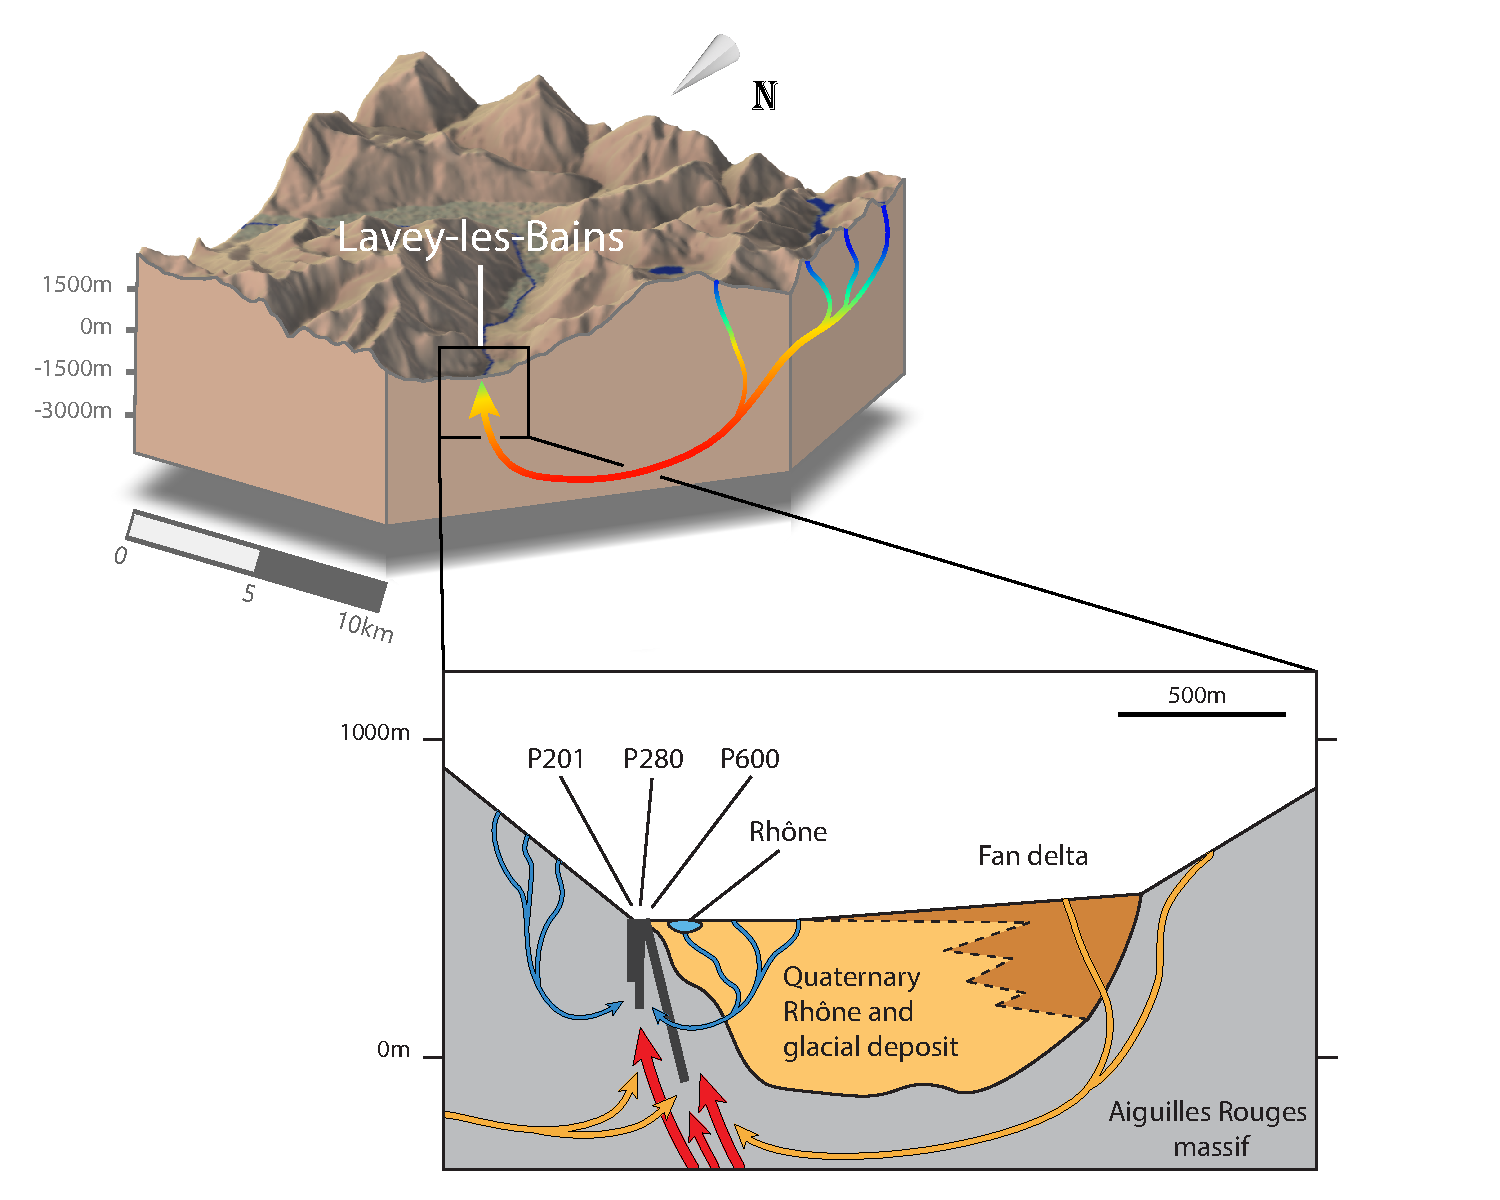
\includegraphics[width=1\textwidth]{chapters/01_introduction/Lavey_diss.pdf}
\end{center}
\caption{Groundwater pathways in the thermal system of Lavey-les-Bains.
Water infiltrates in the surrounding mountains and circulates to depths of several kilometers, where temperatures of approximately \SI{110}{\celsius} are expected \citep{sonney2009numerical, wanner2019quantification}.
Heated water then rises back toward the surface, gradually mixing with shallower groundwater.
Modified from \cite{sonney2009numerical}.}
\label{fig:intro_Lavey}
\end{figure}
\clearpage
}

Lavey-les-Bains is situated in the Rhône Valley between the Aiguilles Rouges Massif and the Morcles Nappe, a large recumbent fold that dominates the regional geological structure \citep{gouffon2024tectonic}.
The area is characterized by a fractured crystalline basement, primarily composed of gneiss, which facilitates deep groundwater circulation \citep{swisstopo2024lavey1, bianchetti1994hydrogeologie, sonney2009numerical}.
Surface water infiltrates through these fractures in the surrounding mountains, percolating to depths where it is progressively heated before resurfacing as thermal springs (Figure~\ref{fig:intro_Lavey}).

This geothermal field exhibits strong seasonal hydrological variability, as evidenced by fluctuations in electrical conductivity \citep{sonney2009numerical}, as well as in gas concentration variations discussed in Chapter~\ref{ch:microbiology}.
While seasonal mixing between deep thermal fluids and shallower groundwater has been observed, its extent, variability, and impact on system dynamics remain poorly constrained.
Despite the importance of fluid dynamics in this system, the microbial communities inhabiting the deep geothermal waters remain largely unexplored.
As the waters are used for thermal spa facilities, microbial investigations have primarily focused on pathogen monitoring, with little attention given to the native subsurface microbial communities that may influence geochemical cycling and fluid evolution.


\section{Outline}
This thesis is divided into five main chapters in order to investigate the interactions between geothermal fluid dynamics, microbial communities, and seismic activity.
Following this introductory chapter, Chapter 2 presents the development of a new methodology for long-term gas monitoring in thermal waters, which provides the basis to rigorously assess geochemically the evolution of a thermal system in time.
Chapters 3 and 4 apply this methodology to investigate the resilience of microbial communities to seasonal hydrological variations and the relationship between fluid geochemistry and seismicity, respectively.
Finally, Chapter 5 synthesizes the results and discusses broader implications, including potential applications of the developed techniques in geothermal research and environmental monitoring.\vspace{10pt}

\textbf{\textit{Chapter 2: New Experimental Approaches Enabling the Continuous Monitoring of Gas Species in Hydrothermal Fluids}} --- This chapter addresses a new methodology to improve long-term gas monitoring in thermal waters using the miniRUEDI system.
The main experimental challenge addressed is the formation of macroscopic water in the analyzed gas phase when its temperature exceeds the ambient temperature, leading to clogging of the miniRUEDI inlet.
To ensure uninterrupted analysis of free gases, two different experimental approaches were developed for two different temperature ranges (up to \SI{65}{\celsius} and over \SI{65}{\celsius}).
The effectiveness of the developed methods was demonstrated by field applications in Lavey-les-Bains (Switzerland) and Beppu (Japan).
This chapter provides the experimental basis for the subsequent application of this technique in chapters 3 and 4.\vspace{10pt}

\textbf{\textit{Chapter 3: Resilience of Deep Aquifer Microbial Communities to Seasonal Hydrological Fluctuations}} --- This chapter examines deep geothermal microbial communities and their response to seasonal variations in groundwater mixing.
By integrating geochemical parameters, dissolved gas concentrations, and isotopic analyses, the mixing ratios of different water components within the thermal system were determined.
The results indicate that while seasonal groundwater recharge influences the mixing dynamics of different water sources, each with its own geochemical signature, microbial community structures remained remarkably stable.
This suggests that temperature gradients, rather than seasonal mixing, are the primary drivers in shaping microbial community composition in the thermal system of Lavey-les-Bains.\vspace{10pt}

\textbf{\textit{Chapter 4: Geochemical Fingerprints of Earthquakes in Alpine Groundwater}} --- This chapter examines the relationship between geothermal fluid geochemistry and seismic activity by analyzing long-term dissolved gas measurements from the miniRUEDI system.
More than \num{250000} gas measurements from two deep wells abstracting thermal water at \SI{200}{\metre} (P201) and at \SI{516}{\metre} (P600) in Lavey-les-Bains were analyzed using a Euclidean distance approach.
The Uclidean distance allows the identification of short-term (several days) geochemical variations against long-term (seasonal) and very short-term (pumping-related) effects.
The results indicate a significant correlation ($>$\SI{60}{\percent}) between short-term geochemical variations and local and regional seismicity in the Canton of Valais, particularly in well P201, while well P600 showed no clear correlation.
Conceptually, these variations are attributed to changes in pore structure and pressure induced by regional seismic events.
This concept may also be applicable to other thermal systems.